\documentclass{standalone}
\usepackage{tikz}
\usetikzlibrary{patterns, positioning}


\begin{document}
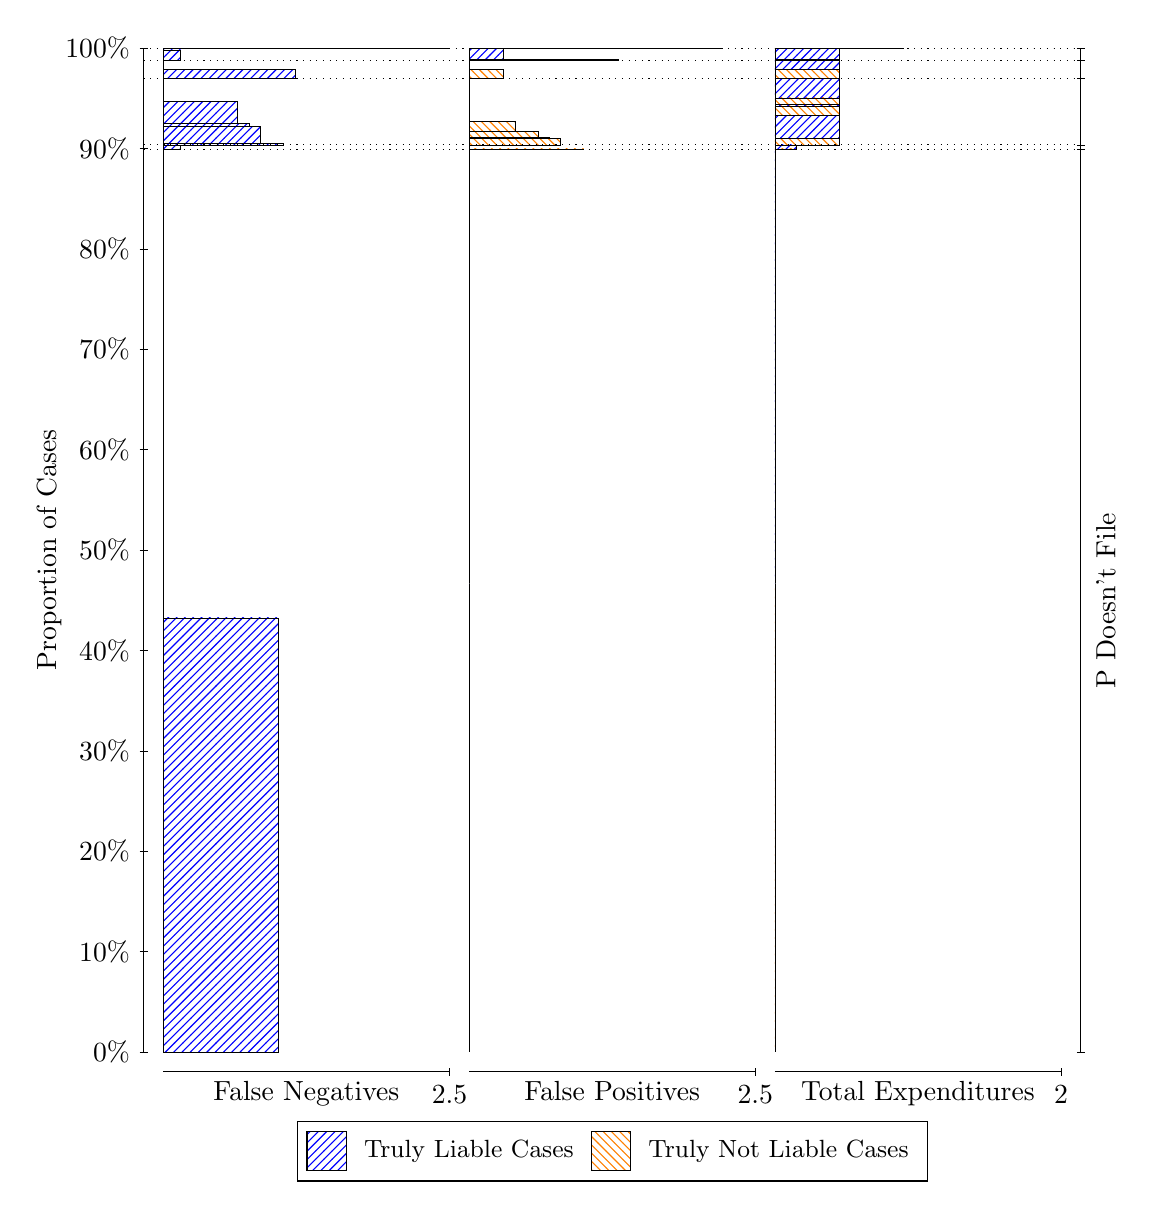
\begin{tikzpicture}
\draw[black, very thin] (1.5,1.75) -- (1.5,14.5);
\node[rotate=90, text=black, anchor=center] at (0.3, 8.125) {Proportion of Cases};
\draw[black, very thin] (1.45,1.75) -- (1.55,1.75);
\node[text=black, anchor=east] at (1.45, 1.75) {0\%};
\draw[black, very thin] (1.45,3.025) -- (1.55,3.025);
\node[text=black, anchor=east] at (1.45, 3.025) {10\%};
\draw[black, very thin] (1.45,4.3) -- (1.55,4.3);
\node[text=black, anchor=east] at (1.45, 4.3) {20\%};
\draw[black, very thin] (1.45,5.575) -- (1.55,5.575);
\node[text=black, anchor=east] at (1.45, 5.575) {30\%};
\draw[black, very thin] (1.45,6.85) -- (1.55,6.85);
\node[text=black, anchor=east] at (1.45, 6.85) {40\%};
\draw[black, very thin] (1.45,8.125) -- (1.55,8.125);
\node[text=black, anchor=east] at (1.45, 8.125) {50\%};
\draw[black, very thin] (1.45,9.4) -- (1.55,9.4);
\node[text=black, anchor=east] at (1.45, 9.4) {60\%};
\draw[black, very thin] (1.45,10.675) -- (1.55,10.675);
\node[text=black, anchor=east] at (1.45, 10.675) {70\%};
\draw[black, very thin] (1.45,11.95) -- (1.55,11.95);
\node[text=black, anchor=east] at (1.45, 11.95) {80\%};
\draw[black, very thin] (1.45,13.225) -- (1.55,13.225);
\node[text=black, anchor=east] at (1.45, 13.225) {90\%};
\draw[black, very thin] (1.45,14.5) -- (1.55,14.5);
\node[text=black, anchor=east] at (1.45, 14.5) {100\%};

\draw[black, very thin] (13.4,1.75) -- (13.4,14.5);
\draw[black, very thin] (13.35,1.75) -- (13.45,1.75);
\node[anchor=west] at (13.35, 1.75) {};
\draw[black, very thin] (13.35,13.212) -- (13.45,13.212);
\node[anchor=west] at (13.35, 13.212) {};
\draw[black, very thin] (13.35,13.27) -- (13.45,13.27);
\node[anchor=west] at (13.35, 13.27) {};
\draw[black, very thin] (13.35,14.118) -- (13.45,14.118);
\node[anchor=west] at (13.35, 14.118) {};
\draw[black, very thin] (13.35,14.342) -- (13.45,14.342);
\node[anchor=west] at (13.35, 14.342) {};
\draw[black, very thin] (13.35,14.491) -- (13.45,14.491);
\node[anchor=west] at (13.35, 14.491) {};
\draw[black, very thin] (13.35,14.494) -- (13.45,14.494);
\node[anchor=west] at (13.35, 14.494) {};
\draw[black, very thin] (13.35,14.5) -- (13.45,14.5);
\node[anchor=west] at (13.35, 14.5) {};

\draw[black, very thin, pattern color=blue, pattern=north east lines] (1.75,1.75) rectangle (3.2033,7.264);
\draw[black, very thin, pattern color=orange, pattern=north west lines] (1.75,7.264) rectangle (1.75,13.212);
\draw[black, very thin, pattern color=blue, pattern=north east lines] (1.75,13.212) rectangle (1.968,13.264);
\draw[black, very thin, pattern color=orange, pattern=north west lines] (1.75,13.264) rectangle (1.75,13.27);
\draw[black, very thin, pattern color=blue, pattern=north east lines] (1.75,13.27) rectangle (3.276,13.29);
\draw[black, very thin, pattern color=blue, pattern=north east lines] (1.75,13.29) rectangle (2.9853,13.503);
\draw[black, very thin, pattern color=blue, pattern=north east lines] (1.75,13.503) rectangle (2.84,13.542);
\draw[black, very thin, pattern color=blue, pattern=north east lines] (1.75,13.542) rectangle (2.6947,13.824);
\draw[black, very thin, pattern color=orange, pattern=north west lines] (1.75,13.824) rectangle (1.75,14.118);
\draw[black, very thin, pattern color=blue, pattern=north east lines] (1.75,14.118) rectangle (3.4213,14.232);
\draw[black, very thin, pattern color=orange, pattern=north west lines] (1.75,14.232) rectangle (1.75,14.342);
\draw[black, very thin, pattern color=blue, pattern=north east lines] (1.75,14.342) rectangle (1.968,14.477);
\draw[black, very thin, pattern color=orange, pattern=north west lines] (1.75,14.477) rectangle (1.75,14.491);
\draw[black, very thin, pattern color=blue, pattern=north east lines] (1.75,14.491) rectangle (5.3833,14.493);
\draw[black, very thin, pattern color=orange, pattern=north west lines] (1.75,14.493) rectangle (1.75,14.494);
\draw[black, very thin, pattern color=orange, pattern=north west lines] (1.75,14.494) rectangle (1.75,14.495);
\draw[black, very thin, pattern color=blue, pattern=north east lines] (1.75,14.495) rectangle (1.75,14.5);
\draw[black, very thin, pattern color=orange, pattern=north west lines] (5.6333,1.75) rectangle (5.6333,7.6978);
\draw[black, very thin, pattern color=blue, pattern=north east lines] (5.6333,7.6978) rectangle (5.6333,13.212);
\draw[black, very thin, pattern color=orange, pattern=north west lines] (5.6333,13.212) rectangle (7.0867,13.218);
\draw[black, very thin, pattern color=blue, pattern=north east lines] (5.6333,13.218) rectangle (5.6333,13.27);
\draw[black, very thin, pattern color=orange, pattern=north west lines] (5.6333,13.27) rectangle (6.796,13.357);
\draw[black, very thin, pattern color=orange, pattern=north west lines] (5.6333,13.357) rectangle (6.6507,13.361);
\draw[black, very thin, pattern color=orange, pattern=north west lines] (5.6333,13.361) rectangle (6.5053,13.438);
\draw[black, very thin, pattern color=orange, pattern=north west lines] (5.6333,13.438) rectangle (6.2147,13.564);
\draw[black, very thin, pattern color=blue, pattern=north east lines] (5.6333,13.564) rectangle (5.6333,14.118);
\draw[black, very thin, pattern color=orange, pattern=north west lines] (5.6333,14.118) rectangle (6.0693,14.229);
\draw[black, very thin, pattern color=blue, pattern=north east lines] (5.6333,14.229) rectangle (5.6333,14.342);
\draw[black, very thin, pattern color=orange, pattern=north west lines] (5.6333,14.342) rectangle (7.5227,14.357);
\draw[black, very thin, pattern color=blue, pattern=north east lines] (5.6333,14.357) rectangle (6.0693,14.491);
\draw[black, very thin, pattern color=orange, pattern=north west lines] (5.6333,14.491) rectangle (5.6333,14.493);
\draw[black, very thin, pattern color=blue, pattern=north east lines] (5.6333,14.493) rectangle (5.6333,14.494);
\draw[black, very thin, pattern color=orange, pattern=north west lines] (5.6333,14.494) rectangle (8.8307,14.495);
\draw[black, very thin, pattern color=blue, pattern=north east lines] (5.6333,14.495) rectangle (7.3773,14.5);
\draw[black, very thin, pattern color=orange, pattern=north west lines] (9.5167,1.75) rectangle (9.5167,7.6978);
\draw[black, very thin, pattern color=blue, pattern=north east lines] (9.5167,7.6978) rectangle (9.5167,13.212);
\draw[black, very thin, pattern color=orange, pattern=north west lines] (9.5167,13.212) rectangle (9.7892,13.218);
\draw[black, very thin, pattern color=blue, pattern=north east lines] (9.5167,13.218) rectangle (9.7892,13.27);
\draw[black, very thin, pattern color=orange, pattern=north west lines] (9.5167,13.27) rectangle (10.334,13.357);
\draw[black, very thin, pattern color=blue, pattern=north east lines] (9.5167,13.357) rectangle (10.334,13.64);
\draw[black, very thin, pattern color=orange, pattern=north west lines] (9.5167,13.64) rectangle (10.334,13.765);
\draw[black, very thin, pattern color=blue, pattern=north east lines] (9.5167,13.765) rectangle (10.334,13.785);
\draw[black, very thin, pattern color=orange, pattern=north west lines] (9.5167,13.785) rectangle (10.334,13.866);
\draw[black, very thin, pattern color=blue, pattern=north east lines] (9.5167,13.866) rectangle (10.334,14.118);
\draw[black, very thin, pattern color=orange, pattern=north west lines] (9.5167,14.118) rectangle (10.334,14.229);
\draw[black, very thin, pattern color=blue, pattern=north east lines] (9.5167,14.229) rectangle (10.334,14.342);
\draw[black, very thin, pattern color=orange, pattern=north west lines] (9.5167,14.342) rectangle (10.334,14.357);
\draw[black, very thin, pattern color=blue, pattern=north east lines] (9.5167,14.357) rectangle (10.334,14.491);
\draw[black, very thin, pattern color=orange, pattern=north west lines] (9.5167,14.491) rectangle (11.152,14.493);
\draw[black, very thin, pattern color=blue, pattern=north east lines] (9.5167,14.493) rectangle (11.152,14.494);
\draw[black, very thin, pattern color=orange, pattern=north west lines] (9.5167,14.494) rectangle (11.152,14.495);
\draw[black, very thin, pattern color=blue, pattern=north east lines] (9.5167,14.495) rectangle (11.152,14.5);
\draw[black, dotted] (1.5,13.212) -- (13.4,13.212);
\draw[black, dotted] (1.5,13.27) -- (13.4,13.27);
\draw[black, dotted] (1.5,14.118) -- (13.4,14.118);
\draw[black, dotted] (1.5,14.342) -- (13.4,14.342);
\draw[black, dotted] (1.5,14.491) -- (13.4,14.491);
\draw[black, dotted] (1.5,14.494) -- (13.4,14.494);
\draw[black, very thin] (1.75,1.5) -- (5.3833,1.5);
\node[text=black, anchor=north] at (3.5667, 1.5) {False Negatives};
\draw[black, very thin] (5.3833,1.45) -- (5.3833,1.55);
\node[text=black, anchor=north] at (5.3833, 1.45) {2.5};

\draw[black, very thin] (5.6333,1.5) -- (9.2667,1.5);
\node[text=black, anchor=north] at (7.45, 1.5) {False Positives};
\draw[black, very thin] (9.2667,1.45) -- (9.2667,1.55);
\node[text=black, anchor=north] at (9.2667, 1.45) {2.5};

\draw[black, very thin] (9.5167,1.5) -- (13.15,1.5);
\node[text=black, anchor=north] at (11.333, 1.5) {Total Expenditures};
\draw[black, very thin] (13.15,1.45) -- (13.15,1.55);
\node[text=black, anchor=north] at (13.15, 1.45) {2};

\node[text=black, centered, rotate=90] at (13.72, 7.4809) {P Doesn't File};







\draw (7.449999999999999,1.5) node[draw=none] (baseCoordinate) {};
\begin{scope}[align=center]
        \matrix[scale=0.5, draw=black, below=0.5cm of baseCoordinate, nodes={draw}, column sep=0.1cm]{
            \node[rectangle, draw, minimum width=0.5cm, minimum height=0.5cm, pattern color=blue, pattern=north east lines] {}; &
            \node[draw=none, font=\small, text=black] (B) {Truly Liable Cases}; &
            \node[rectangle, draw, minimum width=0.5cm, minimum height=0.5cm, pattern color=orange, pattern=north west lines] {}; &
            \node[draw=none, font=\small, text=black] (B) {Truly Not Liable Cases}; \\
            };
\end{scope}

\end{tikzpicture}
\end{document}